\documentclass{article}
\usepackage{tikz}
\usetikzlibrary{positioning, arrows.meta, calc}
\usepackage{subcaption}

\begin{document}
\begin{figure}
\begin{subfigure}{0.4\linewidth}
\begin{center}
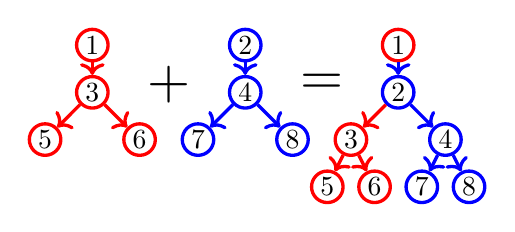
\begin{tikzpicture}[
  scale=0.5,
  level distance=1.2cm,
  every node/.style={circle,draw,minimum size=4mm,inner sep=0pt},
  level 1/.style={sibling distance=12mm},
  level 2/.style={sibling distance=24mm},
  level 3/.style={sibling distance=12mm},
  rededge/.style={draw=red, very thick, ->},
  blueedge/.style={draw=blue, very thick, ->},
  graynode/.style={fill=gray!30}
]

\node (t2) at (0,0) [blueedge] {2}
  child[blueedge] {node {4}
    child {node {7}}
    child {node {8}}
  };

\node[left=1.5cm of t2] (t1) [rededge] {1}
  child[rededge] {node {3}
    child {node {5}}
    child {node {6}}
  };

\node[right=1.5cm of t2, rededge] (t3) {1}
  child [blueedge] {node {2}
    child [rededge] {node {3}
      child {node {5}}
      child {node {6}}
    }
    child [blueedge] {node {4}
      child {node {7}}
      child {node {8}}
    }
  };


\node at ($(t1)!0.5!(t2) + (0,-1.0)$) [draw=none, scale=2] {+};

\node at ($(t2)!0.5!(t3) + (0,-1.0)$) [draw=none, scale=2] {=};

\end{tikzpicture}
\end{center}
\caption{This is the example of a worst case scenario, where all values in the left hand side are larger than the right hand side.}
\end{subfigure}
\hfill
\begin{subfigure}{0.4\linewidth}
\begin{center}
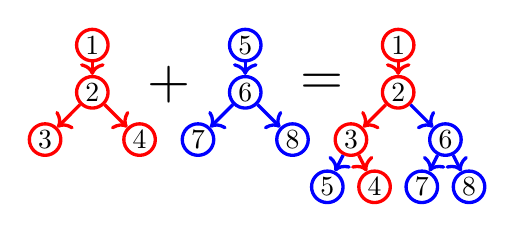
\begin{tikzpicture}[
  scale=0.5,
  level distance=1.2cm,
  every node/.style={circle,draw,minimum size=4mm,inner sep=0pt},
  level 1/.style={sibling distance=12mm},
  level 2/.style={sibling distance=24mm},
  level 3/.style={sibling distance=12mm},
  rededge/.style={draw=red, very thick, ->},
  blueedge/.style={draw=blue, very thick, ->},
  graynode/.style={fill=gray!30}
]

\node (t2) at (0,0) [blueedge] {5}
  child[blueedge] {node {6}
    child {node {7}}
    child {node {8}}
  };

\node[left=1.5cm of t2] (t1) [rededge] {1}
  child[rededge] {node {2}
    child {node {3}}
    child {node {4}}
  };

\node[right=1.5cm of t2, rededge] (t3) {1}
  child [rededge] {node {2}
    child [rededge] {node {3}
      child [blueedge] {node {5}}
      child [rededge] {node {4}}
    }
    child [blueedge] {node {6}
      child {node {7}}
      child {node {8}}
    }
  };


\node at ($(t1)!0.5!(t2) + (0,-1.0)$) [draw=none, scale=2] {+};

\node at ($(t2)!0.5!(t3) + (0,-1.0)$) [draw=none, scale=2] {=};

\end{tikzpicture}
\end{center}
\caption{This is the example of a worst case scenario, where all values in the left hand side are larger than the right hand side.}
\end{subfigure}
\begin{center}
\begin{subfigure}{0.8\linewidth}
\begin{center}
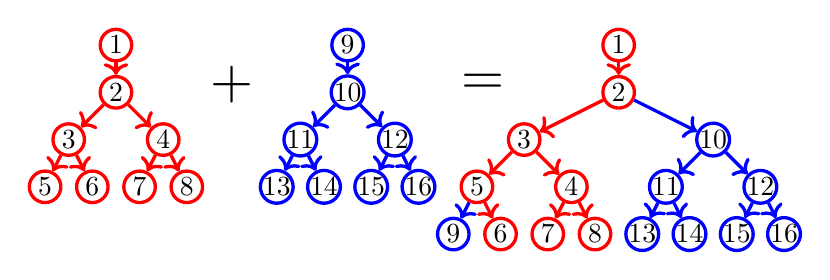
\begin{tikzpicture}[
  scale=0.5,
  level distance=1.2cm,
  every node/.style={circle,draw,minimum size=4mm,inner sep=0pt},
  level 1/.style={sibling distance=12mm},
  level 2/.style={sibling distance=24mm},
  level 3/.style={sibling distance=12mm},
  rededge/.style={draw=red, very thick, ->},
  blueedge/.style={draw=blue, very thick, ->},
  graynode/.style={fill=gray!30}
]

\node (t2) at (0,0) [blueedge] {9}
  child[blueedge] {node {10}
    child {node {11}
      child {node {13}}
      child {node {14}}
    }
    child {node {12}
      child {node {15}}
      child {node {16}}
    }
  };


\node[left=2.5cm of t2] (t1) [rededge] {1}
  child[rededge] {node {2}
    child {node {3}
      child {node {5}}
      child {node {6}}
    }
    child {node {4}
      child {node {7}}
      child {node {8}}
    }
  };

\node[right=3cm of t2, rededge,
] (t3) {1}
  child [rededge] {node {2}
    child [sibling distance=48mm] {node {3}
      child [sibling distance=24mm] {node {5}
        child [sibling distance=12mm, blueedge] {node {9}}
        child [sibling distance=12mm] {node {6}}
      }
      child [sibling distance=24mm] {node {4}
        child [sibling distance=12mm]{node {7}}
        child [sibling distance=12mm]{node {8}}
      }
    }
    child [sibling distance=48mm, blueedge] {node {10}
      child [sibling distance=24mm]{node {11}
        child [sibling distance=12mm]{node {13}}
        child [sibling distance=12mm]{node {14}}
      }
      child [sibling distance=24mm]{node {12}
        child [sibling distance=12mm]{node {15}}
        child [sibling distance=12mm]{node {16}}
      }
    }
  };


\node at ($(t1)!0.5!(t2) + (0,-1.0)$) [draw=none, scale=2] {+};

\node at ($(t2)!0.5!(t3) + (0,-1.0)$) [draw=none, scale=2] {=};

\end{tikzpicture}
\end{center}
\caption{This is the example of a worst case scenario, where all values in the left hand side are larger than the right hand side.}
\end{subfigure}
\end{center}

\caption{Examples of Linking two $\hat{T}_2$ tree, though this these two }
\end{figure}


\end{document}
